\ylDisplay{Mõõteriistad} % Ülesande nimi
{Koit Timpmann} % Autor
{lõppvoor} % Voor
{2006} % Aasta
{G 1} % Ülesande nr.
{1} % Raskustase
{
% Teema: Elektriahelad
\ifStatement
Vooluringis on ampermeeter ja voltmeeter ühendatud jadamisi. Klemmidele on rakendatud pinge $U = \SI{9}{V}$. Kui voltmeetriga ühendada rööbiti takisti $R$, väheneb voltmeetri näit kaks korda, ampermeetri näit aga suureneb kaks korda. Kui suurt pinget näitas voltmeeter enne ja pärast takisti ühendamist?

\begin{center}
	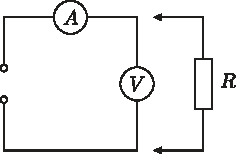
\includegraphics[width=0.5\linewidth]{2006-v3g-01-yl}
\end{center}
\fi


\ifHint
Ampermeetri ja voltmeetri pingete summa peab olema võrdne klemmidele rakendatava pingega nii enne kui ka pärast takisti ühendamist.
\fi


\ifSolution
Olgu alguses ampermeetri ja voltmeetri pinged vastavalt $U_A$ ja $U_V$. Jadaühenduse korral kehtib
\[
U_A + U_V = \SI{9}{V}.
\]
Peale takisti lisamist suurenes ampermeetrit läbiv vool ja seega ka pinge kaks korda. Teisisõnu ampermeetri uus pinge oli $2U_A$. Pinge voltmeetril aga vähenes kaks korda ja oli $\num{0,5}U_V$. Kirchhoffi pinge seaduse kohaselt
\[
2U_A + \num{0,5}U_V = \SI{9}{V}.
\]
Lahendades kahest võrrandist koosneva võrrandisüsteemi, saame $U_A = \SI{3}{V}$ ja $U_V = \SI{6}{V}$. Seega voltmeetril pinge oli alguses \SI{6}{V} ning lõpus \SI{3}{V}.
\fi
}